% 第15章第3节：秩k逼近（子空间选择与迹极值、截断SVD的构造、最佳误差与最优性、最优解的唯一性）。

\section{秩\texorpdfstring{$k$}{k}逼近}
\label{sec:ls-low-rank-approximation}
\label{sec:ls-low-rank-solve}
\label{sec:ls-full-svd-solve}
\label{sec:matrix-analysis-svd-low-rank}

把共同的重建方向由一条直线扩展为$k$维子空间。与秩一情形一样，先固定子空间求系数，再选择子空间本身；用子空间的标准正交基，保留量写成一个迹，选子空间就成为迹的极值问题。由奇异值分解可以写出这个问题的解，即截断SVD；随后在Frobenius范数与谱范数下证明它的最优性，并讨论最优解何时唯一。

\subsection{子空间选择与迹极值}
\label{sec:ls-low-rank-projection-error}
\label{sec:ls-rank-k-trace}

先固定一个$k$维子空间，问最好的重建是什么。以列标准正交的$\bm Y\in\mathbb R^{m\times k}$表示这个子空间，$\bm Y^\top\bm Y=\bm I_k$；这里不用字母$\bm V$，以免与右奇异向量矩阵混淆。列都落在$\operatorname{range}(\bm Y)$中的矩阵恰好是$\bm X=\bm Y\bm C$，$\bm C\in\mathbb R^{k\times d}$的第$j$列是$\bm x_j$在这组基下的系数。由第~\ref{chap:normed-inner-product-spaces}章的投影矩阵，$\bm Y\bm Y^\top$是到$\operatorname{range}(\bm Y)$的正交投影。

\begin{lemma}[固定子空间时的正交误差分解]
\label{lem:ls-low-rank-projection-error}
设$\bm Y\in\mathbb R^{m\times k}$满足$\bm Y^\top\bm Y=\bm I_k$，则对任意$\bm C\in\mathbb R^{k\times d}$，
\begin{equation}
 \begin{aligned}
 \lVert\bm A-\bm Y\bm C\rVert_{\mathrm F}^2
 &=\lVert(\bm I-\bm Y\bm Y^\top)\bm A\rVert_{\mathrm F}^2\\
 &\qquad+\lVert\bm Y^\top\bm A-\bm C\rVert_{\mathrm F}^2,
 \end{aligned}
 \label{eq:ls-low-rank-projection-split}
\end{equation}
并且
\[
 \lVert(\bm I-\bm Y\bm Y^\top)\bm A\rVert_{\mathrm F}^2
 =\lVert\bm A\rVert_{\mathrm F}^2-\operatorname{tr}(\bm Y^\top\bm A\bm A^\top\bm Y).
\]
因此固定子空间时，最优系数唯一，为$\bm C=\bm Y^\top\bm A$，最优重建是正交投影$\bm Y\bm Y^\top\bm A$。
\end{lemma}
\begin{proof}
写$\bm A-\bm Y\bm C=(\bm I-\bm Y\bm Y^\top)\bm A+\bm Y(\bm Y^\top\bm A-\bm C)$。逐列看，第$j$列是$\bm r_j=(\bm I-\bm Y\bm Y^\top)\bm a_j$与$\bm Y\bm z_j$之和，其中$\bm z_j$是$\bm Y^\top\bm A-\bm C$的第$j$列。二者正交：
\[
 \bm r_j^\top\bm Y\bm z_j=\bm a_j^\top(\bm I-\bm Y\bm Y^\top)\bm Y\bm z_j
 =\bm a_j^\top(\bm Y-\bm Y\bm Y^\top\bm Y)\bm z_j=0 ,
\]
这里用到$\bm Y^\top\bm Y=\bm I_k$。又$\lVert\bm Y\bm z_j\rVert_2^2=\bm z_j^\top\bm Y^\top\bm Y\bm z_j=\lVert\bm z_j\rVert_2^2$。由勾股定理，第$j$列的平方长度是$\lVert\bm r_j\rVert_2^2+\lVert\bm z_j\rVert_2^2$；对$j$求和即得式~\eqref{eq:ls-low-rank-projection-split}。

对第二式，同样把$\bm a_j$分解为$\bm Y\bm Y^\top\bm a_j$与$\bm r_j$两个正交部分，得$\lVert\bm r_j\rVert_2^2=\lVert\bm a_j\rVert_2^2-\lVert\bm Y^\top\bm a_j\rVert_2^2$。求和后，
\[
 \sum_j\lVert\bm Y^\top\bm a_j\rVert_2^2=\lVert\bm Y^\top\bm A\rVert_{\mathrm F}^2
 =\operatorname{tr}(\bm Y^\top\bm A\bm A^\top\bm Y).
\]
最后，式~\eqref{eq:ls-low-rank-projection-split}右端第一项与$\bm C$无关，第二项非负，且当且仅当$\bm C=\bm Y^\top\bm A$时为零。
\end{proof}

于是在固定子空间中，误差等于总平方长度减去保留量$\operatorname{tr}(\bm Y^\top\bm A\bm A^\top\bm Y)$；$k=1$、$\bm Y=\bm u$时，这正是第~\ref{sec:matrix-approximation-rank-one-coefficients}节逐列配方得到的公式。示例~\ref{ex:ls-low-rank-three-columns}中“先投影再计损失”的做法，也正是这个最优重建。共同子空间把$d$个向量各自的最小二乘问题合成了一个矩阵近似问题：子空间共用，系数逐列由投影给出。

这一化归覆盖全部候选矩阵，而不只覆盖事先写成投影形式的矩阵。设$\operatorname{rank}\bm X=s\leq k$。取$\bm X$列空间的一组标准正交基，再在$\mathbb R^m$中补充$k-s$个与之正交的单位向量（$k\leq m$，所以可以补齐），排成$\bm Y$。则$\bm X$的列都落在$\operatorname{range}(\bm Y)$中，$\bm X=\bm Y\bm C$，其中$\bm C=\bm Y^\top\bm X$。由引理~\ref{lem:ls-low-rank-projection-error}，
\[
 \lVert\bm A-\bm X\rVert_{\mathrm F}^2\geq\lVert\bm A\rVert_{\mathrm F}^2-\operatorname{tr}(\bm Y^\top\bm A\bm A^\top\bm Y).
\]
反过来，每个列标准正交的$\bm Y$都给出秩不超过$k$的候选$\bm Y\bm Y^\top\bm A$，误差恰为右端。两方面合起来，
\begin{equation}
 \begin{aligned}
 &\min_{\operatorname{rank}\bm X\leq k}\lVert\bm A-\bm X\rVert_{\mathrm F}^2\\
 &\qquad=\lVert\bm A\rVert_{\mathrm F}^2-\max_{\bm Y^\top\bm Y=\bm I_k}\operatorname{tr}(\bm Y^\top\bm A\bm A^\top\bm Y),
 \end{aligned}
 \label{eq:ls-low-rank-subspace-reduction}
\end{equation}
只要右端的最大值存在；最大值的存在与取值由下面的定理~\ref{thm:matrix-analysis-trace-minimum}给出。到这里，“同时选择方向与系数”化成了“选择子空间”。

再看保留量本身。对$\bm Y=[\bm y_1,\ldots,\bm y_k]$按列展开：
\[
 \operatorname{tr}(\bm Y^\top\bm A\bm A^\top\bm Y)
 =\sum_{l=1}^k\bm y_l^\top\bm A\bm A^\top\bm y_l
 =\sum_{l=1}^k\sum_{j=1}^d(\bm y_l^\top\bm a_j)^2 .
\]
迹把$k$个互相垂直方向上的保留量相加，$k=1$时恰好回到上一节的Rayleigh商。它只依赖子空间，不依赖基的选取：把$\bm Y$换成$\bm Y\bm O$（$\bm O$为$k$阶正交矩阵）时，由迹的循环性，$\operatorname{tr}(\bm O^\top\bm Y^\top\bm G\bm Y\bm O)=\operatorname{tr}(\bm Y^\top\bm G\bm Y)$，其中$\bm G=\bm A\bm A^\top$。

据此，由式~\eqref{eq:ls-low-rank-subspace-reduction}，秩$k$逼近归结为下面的\emph{迹极值问题}：
\[
 \text{在}\ \bm Y^\top\bm Y=\bm I_k\ \text{下最大化}\ \operatorname{tr}(\bm Y^\top\bm G\bm Y),\qquad\bm G=\bm A\bm A^\top .
\]
逐列套用Rayleigh--Ritz定理只能得到每一项不超过$\lambda_1(\bm G)$，即总和不超过$k\lambda_1(\bm G)$。这个界没有用到各列互相正交的约束，一般取不到：由定理~\ref{thm:matrix-analysis-rayleigh-ritz}的取等条件，总和等于$k\lambda_1(\bm G)$要求每个$\bm y_l$都落在最大特征值的特征空间中；若$\lambda_1(\bm G)$单重，这个特征空间是一条直线，$k\geq2$时容不下$k$个互相正交的单位向量。

先只比较由$\bm G$的特征向量组成的子空间。设$\bm G$的特征值为$\lambda_1\geq\cdots\geq\lambda_m$，对应标准正交特征向量$\bm q_1,\ldots,\bm q_m$。取$\bm Y=[\bm q_{i_1},\ldots,\bm q_{i_k}]$（下标互不相同），则$\bm y_l^\top\bm G\bm y_l=\lambda_{i_l}$，保留量为$\lambda_{i_1}+\cdots+\lambda_{i_k}$；保留前$k$个特征方向给出最大的特征值和$\sum_{i\leq k}\lambda_i$。这给出一个明确的候选。任意倾斜的子空间会把权重分散到多个特征方向上，它是否仍不能超过这个值，需要下面的定理来回答。

回到示例~\ref{ex:ls-low-rank-three-columns}，$\bm G=\operatorname{diag}(9,4,1)$，前两个特征方向张成$\operatorname{span}\{\bm e_1,\bm e_2\}$，保留量$13$，损失$1$，正是三个坐标平面中最好的一个。一般地，由式~\eqref{eq:ls-svd-transpose-relation}，$\bm A\bm A^\top$的前$k$个特征方向可以取为左奇异向量$\bm u_1,\ldots,\bm u_k$，候选子空间就是$\operatorname{span}\{\bm u_1,\ldots,\bm u_k\}$。

同样的问题可以对任意实对称矩阵$\bm S$提出：在$\bm Y^\top\bm Y=\bm I_k$下，$\operatorname{tr}(\bm Y^\top\bm S\bm Y)$能否超过前$k$个特征值之和，又能否低于后$k$个特征值之和？证明的想法是把迹写成特征值的加权和，看清正交约束对权重施加了什么限制。

\begin{theorem}[迹极值]
\label{thm:matrix-analysis-trace-minimum}
设$\bm S\in\mathbb R^{m\times m}$实对称，特征值$\lambda_1\geq\cdots\geq\lambda_m$，对应标准正交特征向量$\bm q_1,\ldots,\bm q_m$，$1\leq k\leq m$。对满足$\bm Y^\top\bm Y=\bm I_k$的$\bm Y\in\mathbb R^{m\times k}$，
\begin{equation}
 \sum_{i=m-k+1}^{m}\lambda_i\leq\operatorname{tr}(\bm Y^\top\bm S\bm Y)\leq\sum_{i=1}^{k}\lambda_i,
 \label{eq:matrix-analysis-trace-minimum}
\end{equation}
上界由$\bm Y=[\bm q_1,\ldots,\bm q_k]$取到，下界由$\bm Y=[\bm q_{m-k+1},\ldots,\bm q_m]$取到。若$k<m$且$\lambda_k>\lambda_{k+1}$，则上界取等当且仅当$\operatorname{range}(\bm Y)=\operatorname{span}\{\bm q_1,\ldots,\bm q_k\}$。
\end{theorem}
\begin{proof}
由谱定理，$\bm S=\sum_i\lambda_i\bm q_i\bm q_i^\top$，故
\[
 \operatorname{tr}(\bm Y^\top\bm S\bm Y)
 =\sum_{i=1}^m\lambda_i\operatorname{tr}(\bm Y^\top\bm q_i\bm q_i^\top\bm Y)
 =\sum_{i=1}^m\lambda_iw_i,
\]
其中$w_i=\lVert\bm Y^\top\bm q_i\rVert_2^2$。权重受两条限制。第一，$\bm P=\bm Y\bm Y^\top$是到$\operatorname{range}(\bm Y)$的正交投影，$w_i=\bm q_i^\top\bm P\bm q_i=\bm q_i^\top\bm P^\top\bm P\bm q_i=\lVert\bm P\bm q_i\rVert_2^2$；正交投影不增加长度，所以$0\leq w_i\leq\lVert\bm q_i\rVert_2^2=1$。第二，记$\bm Q=[\bm q_1,\ldots,\bm q_m]$，它是正交矩阵，右乘正交矩阵不改变Frobenius范数，于是
\[
 \sum_{i=1}^mw_i=\lVert\bm Y^\top\bm Q\rVert_{\mathrm F}^2=\lVert\bm Y^\top\rVert_{\mathrm F}^2=\operatorname{tr}(\bm Y^\top\bm Y)=k .
\]
也就是说，总量为$k$的权重分配给各个特征值，每个特征值至多分到$1$。

直观上，要使加权和最大，应把权重全部放在最大的$k$个特征值上。用$\lambda_k$作为分界，可以把这一直观写成恒等式：
\[
 \begin{aligned}
 \sum_{i=1}^m\lambda_iw_i-\sum_{i=1}^k\lambda_i
 &=\sum_{i\leq k}(\lambda_i-\lambda_k)(w_i-1)+\sum_{i>k}(\lambda_i-\lambda_k)w_i\\
 &\qquad+\lambda_k\Bigl(\sum_{i=1}^mw_i-k\Bigr).
 \end{aligned}
\]
展开右端即可核对。最后一项因$\sum_iw_i=k$而为零。$i\leq k$时$\lambda_i-\lambda_k\geq0$、$w_i-1\leq0$；$i>k$时$\lambda_i-\lambda_k\leq0$、$w_i\geq0$。所以右端每一项都不大于零，上界成立。$\bm Y=[\bm q_1,\ldots,\bm q_k]$时$w_i$在$i\leq k$时为$1$、其余为$0$，迹等于$\sum_{i\leq k}\lambda_i$。

取等条件也可以从这个恒等式读出。若$\lambda_k>\lambda_{k+1}$，则$i>k$时$\lambda_i-\lambda_k<0$，上界取等迫使$w_i=0$，即$\bm Y^\top\bm q_i=\bm0$。于是$\operatorname{range}(\bm Y)$与$\bm q_{k+1},\ldots,\bm q_m$都正交，含于$\operatorname{span}\{\bm q_1,\ldots,\bm q_k\}$；两者都是$k$维的，所以相等。反之，若$\operatorname{range}(\bm Y)=\operatorname{span}\{\bm q_1,\ldots,\bm q_k\}$，则$i\leq k$时$\bm P\bm q_i=\bm q_i$、$i>k$时$\bm P\bm q_i=\bm0$，迹等于上界。

下界由上界得到。$-\bm S$的特征值按降序为$-\lambda_m\geq\cdots\geq-\lambda_1$，对应特征向量依次为$\bm q_m,\ldots,\bm q_1$。对$-\bm S$应用上界，得$-\operatorname{tr}(\bm Y^\top\bm S\bm Y)\leq-\sum_{i=m-k+1}^m\lambda_i$，等号在$\bm Y=[\bm q_{m-k+1},\ldots,\bm q_m]$时成立。
\end{proof}

回到低秩逼近，取$\bm S=\bm G=\bm A\bm A^\top$。它的特征值是$\sigma_1^2\geq\cdots\geq\sigma_r^2$，再补上$m-r$个零；$k<r$时前$k$个之和为$\sum_{i\leq k}\sigma_i^2$。于是任意$k$维子空间最多保留$\sum_{i=1}^k\sigma_i^2$，式~\eqref{eq:ls-low-rank-subspace-reduction}右端的最大值存在，并由$\operatorname{span}\{\bm u_1,\ldots,\bm u_k\}$取到。在示例~\ref{ex:ls-low-rank-three-columns}中，这确认任意倾斜平面的保留量都不超过$13$，坐标平面$\operatorname{span}\{\bm e_1,\bm e_2\}$已是最优的平面。

对一般的对称矩阵$\bm S$，迹极值界照样成立，但只有在当前这种半正定的Gram情形，迹才表示投影保留的长度平方。下一小节把最优子空间上的投影重建写成具体的矩阵。

\subsection{截断SVD的构造}
\label{sec:ls-truncated-svd-construction}

\paragraph{主要思想}

设$\bm A$的奇异值分解写成和式~\eqref{eq:matrix-analysis-svd-rank-one-sum}，$\bm A=\sum_{i=1}^r\sigma_i\bm u_i\bm v_i^\top$，其中$r=\operatorname{rank}\bm A$，$\sigma_1\geq\cdots\geq\sigma_r>0$。上一小节说明，$1\leq k<r$时最优子空间可取为$\operatorname{span}\{\bm u_1,\ldots,\bm u_k\}$，即$\bm Y=\bm U_k=[\bm u_1,\ldots,\bm u_k]$。由$\bm U_k^\top\bm u_i$在$i\leq k$时等于$\bm e_i$、在$i>k$时等于$\bm0$，这个子空间上的最优重建是
\[
 \begin{aligned}
 \bm U_k\bm U_k^\top\bm A
 &=\sum_{i=1}^r\sigma_i\bm U_k(\bm U_k^\top\bm u_i)\bm v_i^\top\\
 &=\sum_{i=1}^k\sigma_i\bm u_i\bm v_i^\top .
 \end{aligned}
\]
也就是说，把$\bm A$的各列正交投影到前$k$个左奇异方向上，等于只保留SVD和式的前$k$项。

把这个由子空间优化推导出的矩阵记下来。对整数$k\geq0$，称
\begin{equation}
\begin{gathered}
\bm A_k=\sum_{i=1}^{\min(k,r)}\sigma_i\bm u_i\bm v_i^\top
 =\bm U_k\bm\Sigma_k\bm V_k^\top\\
k\geq0
\end{gathered}
\label{eq:matrix-analysis-truncated-svd}
\end{equation}
为$\bm A$的\term{截断SVD}（truncated SVD），其中$k\leq r$时$\bm\Sigma_k=\operatorname{diag}(\sigma_1,\ldots,\sigma_k)$，$\bm V_k=[\bm v_1,\ldots,\bm v_k]$。两种边界情形与第~\ref{sec:matrix-approximation-problem}节的直接回答一致：$k=0$时和式为空，$\bm A_0=\bm0$；$k\geq r$时保留了全部项，$\bm A_k=\bm A$。

$k\leq r$时，$\bm A_k\bm v_i=\sigma_i\bm u_i$（$i\leq k$），而$\bm A_k$与$\bm v_{k+1},\ldots,\bm v_d$的作用为零，所以列空间恰为$\operatorname{span}\{\bm u_1,\ldots,\bm u_k\}$，$\operatorname{rank}\bm A_k=k$，满足秩约束。

\paragraph{算法实现与算例}

给定已经求出的SVD，截断SVD的计算分三步。第一，核对$k$是满足$0\leq k\leq\min(m,d)$的整数，$k\geq r$时直接返回$\bm A$，$k=0$时返回零矩阵。第二，按奇异值非增的顺序读取前$k$个奇异值及配对的左右奇异向量；配对不能打乱，因为每一项$\sigma_i\bm u_i\bm v_i^\top$都要求$\bm A\bm v_i=\sigma_i\bm u_i$。第三，求外积和。若只需要压缩存储，就保留$\bm U_k$、$\sigma_1,\ldots,\sigma_k$与$\bm V_k$三个小因子，不必形成$m\times d$的矩阵；需要核验时，再由因子相乘求出重建误差。

\begin{example}[对角矩阵的截断]
\label{ex:ls-truncated-svd-diagonal}
仍取$\bm A=\operatorname{diag}(3,2,1)$，奇异值为$3,2,1$，可取$\bm u_i=\bm v_i=\bm e_i$。截断得
\[
 \bm A_1=\operatorname{diag}(3,0,0),\qquad\bm A_2=\operatorname{diag}(3,2,0).
\]
$\bm A-\bm A_1=\operatorname{diag}(0,2,1)$，平方误差$2^2+1^2=5$，谱范数误差$2$；$\bm A-\bm A_2=\operatorname{diag}(0,0,1)$，平方误差$1$，谱范数误差$1$。平方误差$5,1$与示例~\ref{ex:ls-low-rank-three-columns}中最佳坐标直线、坐标平面的损失一致。
\end{example}

对角矩阵的奇异方向就是坐标方向。下面的例子中奇异方向是倾斜的，而且有两个相等的奇异值，可以看到截断位置处的重奇异值带来的变化。

\begin{example}[有重奇异值的三阶截断]
\label{ex:matrix-approximation-truncated-three-by-three}
取
\[
 \bm A=\begin{bmatrix}3&2&0\\2&3&0\\0&0&1\end{bmatrix}.
\]
先核验奇异方向。令$\bm u_1=(1,1,0)^\top/\sqrt2$、$\bm u_2=(1,-1,0)^\top/\sqrt2$、$\bm u_3=(0,0,1)^\top$，它们标准正交，且$\bm A\bm u_1=5\bm u_1$、$\bm A\bm u_2=\bm u_2$、$\bm A\bm u_3=\bm u_3$。$\bm A$对称、特征值非负，所以可取$\bm v_i=\bm u_i$，奇异值为$5,1,1$。

取$k=1$，
\[
 \bm A_1=5\bm u_1\bm u_1^\top=\frac52\begin{bmatrix}1&1&0\\1&1&0\\0&0&0\end{bmatrix},\qquad
 \bm A-\bm A_1=\begin{bmatrix}1/2&-1/2&0\\-1/2&1/2&0\\0&0&1\end{bmatrix}.
\]
左上四项均为$5/2$，其余为零。残差的Frobenius范数平方为$4\times\frac14+1=2$，即$\lVert\bm A-\bm A_1\rVert_{\mathrm F}=\sqrt2$。残差等于$\bm u_2\bm u_2^\top+\bm u_3\bm u_3^\top$，是到$\operatorname{span}\{\bm u_2,\bm u_3\}$的正交投影，它把该平面内的单位向量原样送出，把$\bm u_1$送到零，所以谱范数为$1$。

取$k=2$并保留第二方向，得到
\[
 \bm A_2=\bm A_1+\bm u_2\bm u_2^\top=\begin{bmatrix}3&2&0\\2&3&0\\0&0&0\end{bmatrix},
 \qquad\bm A-\bm A_2=\bm e_3\bm e_3^\top ,
\]
残差的两种范数都是$1$。由于$\sigma_2=\sigma_3$，把$\bm u_2$与$\bm u_3$的次序交换也是$\bm A$的一个SVD，按它截断得到$\bm A_2'=\bm A_1+\bm u_3\bm u_3^\top$，残差$\bm u_2\bm u_2^\top$的两种范数同样为$1$。$\bm A_2\neq\bm A_2'$而误差相同，这预示截断位置处奇异值重复时最优矩阵不唯一。
\end{example}

图~\ref{fig:ls-low-rank-truncation}画出截断的几何：单位圆经$\bm A$变成椭圆，秩一近似把椭圆压成主轴方向的线段，残留的谱范数误差恰为舍弃的$\sigma_2$。

\begin{figure*}[htbp]
  \centering
  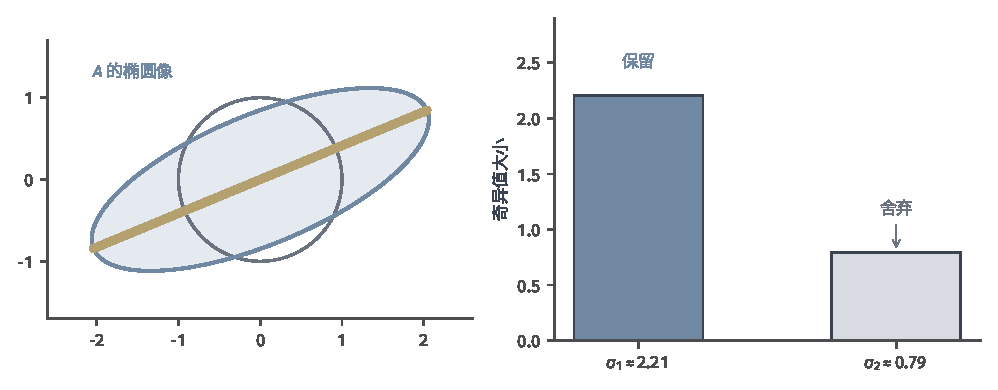
\includegraphics[width=168.998mm]{figures/00-shared/mathematical-preliminaries-upper/02-linear-spaces/matplotlib/ls-low-rank-truncation/ls-low-rank-truncation.pdf}
  \caption{低秩截断的几何。$\bm A=\left[\begin{smallmatrix}2&0.5\\0.5&1\end{smallmatrix}\right]$，
  灰圆为单位圆，蓝椭圆为$\bm A$的像。左：黄粗线段为秩一近似$\bm A_1=\sigma_1\bm v_1\bm v_1^\top$
  的像，椭圆被压成长$2\sigma_1$的线段；右：$\sigma_1\approx2.21$（保留）、$\sigma_2\approx0.79$
  （舍弃），算子范数误差$\lVert\bm A-\bm A_1\rVert_2=\sigma_2$。$\sigma_{1,2}=(3\pm\sqrt2)/2$。
  固定复算。}
  \label{fig:ls-low-rank-truncation}
\end{figure*}

\paragraph{算法分析}

截断SVD的好处还在于表示代价。直接存储$\bm A$需要$md$个数；保存因子$\bm U_k$、$\sigma_1,\ldots,\sigma_k$与$\bm V_k$只需$k(m+d+1)$个数。按$\bm A_k\bm x=\bm U_k\bigl(\bm\Sigma_k(\bm V_k^\top\bm x)\bigr)$的顺序乘向量，依次需要约$dk$、$k$、$mk$次乘法，共$O(k(m+d))$次运算，而直接用$\bm A$乘向量需要$O(md)$次。例如$m=d=1000$、$k=10$时，存储由$10^6$个数降为$20010$个数。

这些是表示与后续作用的代价，不包括计算SVD本身的代价；后者取决于所用的数值算法，本书不作分析。还要注意用途：第~\ref{chap:solution-error-regularization}章的截断SVD求解也用到$\bm A_k$，但那里是用它的伪逆稳定地求解方程；这里$\bm A_k$本身就是要评价的近似对象，评价标准是重建误差。

\subsection{最佳误差与最优性}
\label{sec:ls-truncated-svd-optimality}

先计算截断SVD的实际误差，再比较全部秩不超过$k$的候选。设$0\leq k<r$。余下的$\bm A-\bm A_k=\sum_{i>k}\sigma_i\bm u_i\bm v_i^\top$仍由两组标准正交向量和降序的正系数$\sigma_{k+1}\geq\cdots\geq\sigma_r$组成，可以照第~\ref{sec:ls-svd-matrix-size}节的方法读出它的大小。

对$\bm x=\sum_{i=1}^dc_i\bm v_i$，$(\bm A-\bm A_k)\bm x=\sum_{i=k+1}^r\sigma_ic_i\bm u_i$，由$\bm u_i$标准正交，
\[
 \lVert(\bm A-\bm A_k)\bm x\rVert_2^2=\sum_{i=k+1}^r\sigma_i^2c_i^2\leq\sigma_{k+1}^2\lVert\bm x\rVert_2^2,
\]
等号在$\bm x=\bm v_{k+1}$时成立。又由$\bm u_i^\top\bm u_j=\delta_{i,j}$，$(\bm A-\bm A_k)^\top(\bm A-\bm A_k)=\sum_{i>k}\sigma_i^2\bm v_i\bm v_i^\top$，取迹得Frobenius范数平方$\sum_{i>k}\sigma_i^2$。于是
\begin{equation}
\begin{gathered}
\lVert\bm A-\bm A_k\rVert_2=\sigma_{k+1}\\
\lVert\bm A-\bm A_k\rVert_{\mathrm F}
 =\Bigl(\sum_{i=k+1}^r\sigma_i^2\Bigr)^{1/2}.
\end{gathered}
\label{eq:ls-truncated-errors}
\end{equation}
Frobenius平方误差也可以由引理~\ref{lem:ls-low-rank-projection-error}读出：$\lVert\bm A\rVert_{\mathrm F}^2-\operatorname{tr}(\bm U_k^\top\bm A\bm A^\top\bm U_k)=\sum_{i\leq r}\sigma_i^2-\sum_{i\leq k}\sigma_i^2$。示例~\ref{ex:matrix-approximation-truncated-three-by-three}中$k=1$时，式~\eqref{eq:ls-truncated-errors}给出$\sqrt{1^2+1^2}=\sqrt2$与$\sigma_2=1$，与直接计算一致。

两种误差记录的内容不同：Frobenius平方误差汇总所有舍弃方向，谱范数误差只记录最坏的单位输入方向。式~\eqref{eq:ls-truncated-errors}只是这一构造的误差，尚需证明其他秩不超过$k$的矩阵不能更小。Frobenius范数的结论由上一小节的化归和迹极值得到；谱范数不能这样处理，因为$\lVert\bm M\rVert_2\leq\lVert\bm M\rVert_{\mathrm F}$，Frobenius误差的下界推不出谱范数误差的下界，需要另作证明。

\begin{theorem}[Eckart--Young--Mirsky最佳低秩逼近]
\label{thm:ls-best-low-rank}
\label{thm:matrix-analysis-best-low-rank}
设$\bm A\in\mathbb R^{m\times d}$的秩为$r$，奇异值为$\sigma_1\geq\cdots\geq\sigma_r>0$。对$0\leq k<r$，
\begin{align}
 \min_{\operatorname{rank}\bm X\leq k}\lVert\bm A-\bm X\rVert_2
 &=\sigma_{k+1},
 \label{eq:matrix-analysis-best-rank-k-spectral}\\
 \min_{\operatorname{rank}\bm X\leq k}\lVert\bm A-\bm X\rVert_{\mathrm F}
 &=\Bigl(\sum_{i=k+1}^r\sigma_i^2\Bigr)^{1/2},
 \label{eq:matrix-analysis-best-rank-k-frobenius}
\end{align}
两个最小值都由截断SVD$\bm A_k$达到。
\end{theorem}
\begin{proof}
由式~\eqref{eq:ls-truncated-errors}，$\bm A_k$的两种误差恰为右端，只需证明任意秩不超过$k$的$\bm X$误差都不更小。$k=0$时只有$\bm X=\bm0$，结论即式~\eqref{eq:ls-truncated-errors}，下设$k\geq1$。

Frobenius情形。按第~\ref{sec:ls-low-rank-projection-error}节的做法，把$\bm X$的列空间补成一个$k$维子空间，取其标准正交基组成$\bm Y$，则$\bm X=\bm Y\bm C$。由引理~\ref{lem:ls-low-rank-projection-error}、定理~\ref{thm:matrix-analysis-trace-minimum}与式~\eqref{eq:matrix-analysis-frobenius-norm}，
\[
 \begin{aligned}
 \lVert\bm A-\bm X\rVert_{\mathrm F}^2
 &\geq\lVert\bm A\rVert_{\mathrm F}^2-\operatorname{tr}(\bm Y^\top\bm A\bm A^\top\bm Y)\\
 &\geq\sum_{i=1}^r\sigma_i^2-\sum_{i=1}^k\sigma_i^2=\sum_{i=k+1}^r\sigma_i^2 .
 \end{aligned}
\]

谱范数情形。由秩零度定理~\ref{thm:ls-rank-nullity}，$\dim\ker\bm X=d-\operatorname{rank}\bm X\geq d-k$。子空间$\operatorname{span}\{\bm v_1,\ldots,\bm v_{k+1}\}$的维数为$k+1$（$k+1\leq r\leq d$）。两者维数之和超过$d$，由维数公式，它们有非零公共向量；取其中的单位向量$\bm x=\sum_{i=1}^{k+1}c_i\bm v_i$，$\sum_ic_i^2=1$。由$\bm X\bm x=\bm0$，
\begin{equation}
 \lVert(\bm A-\bm X)\bm x\rVert_2
 =\lVert\bm A\bm x\rVert_2
 =\Bigl(\sum_{i=1}^{k+1}\sigma_i^2c_i^2\Bigr)^{1/2}
 \geq\sigma_{k+1},
 \label{eq:ls-spectral-lower-bound}
\end{equation}
所以$\lVert\bm A-\bm X\rVert_2\geq\sigma_{k+1}$。
\end{proof}

这一结论最早由Eckart与Young给出\scite{eckart1936}。定理覆盖任意秩不超过$k$的矩阵，而不只覆盖事先选定的投影形式：Frobenius情形借助第~\ref{sec:ls-low-rank-projection-error}节的化归把任意候选归入某个子空间，谱范数情形则直接利用候选矩阵的核。两种范数下的最小误差都由舍弃的奇异值决定：谱范数看最大的舍弃值$\sigma_{k+1}$，Frobenius范数看全部舍弃值的平方和。

\subsection{最优解的唯一性}
\label{sec:matrix-approximation-low-rank-uniqueness}

最小误差唯一，达到最小误差的矩阵却未必唯一。在有效的秩预算$1\leq k<r$下，Frobenius情形的唯一性由迹极值的取等条件决定，关键是截断位置两侧的奇异值是否有间隙。

\begin{theorem}[Frobenius最佳逼近的唯一性]
\label{thm:ls-best-low-rank-uniqueness}
设$1\leq k<r$且$\sigma_k>\sigma_{k+1}$，则$\bm A_k$是$\min_{\operatorname{rank}\bm X\leq k}\lVert\bm A-\bm X\rVert_{\mathrm F}$的唯一最优解。
\end{theorem}
\begin{proof}
设$\bm X$达到最小值，按定理~\ref{thm:ls-best-low-rank}的证明取$\bm Y$，写$\bm X=\bm Y\bm C$。证明中的两个不等号都须取等。第一个取等，由式~\eqref{eq:ls-low-rank-projection-split}得$\bm C=\bm Y^\top\bm A$，即$\bm X=\bm Y\bm Y^\top\bm A$。第二个取等，即$\operatorname{tr}(\bm Y^\top\bm A\bm A^\top\bm Y)=\sum_{i\leq k}\sigma_i^2$。$\bm A\bm A^\top$的第$k$与第$k+1$个特征值为$\sigma_k^2>\sigma_{k+1}^2$，由定理~\ref{thm:matrix-analysis-trace-minimum}的取等条件，$\operatorname{range}(\bm Y)=\operatorname{span}\{\bm u_1,\ldots,\bm u_k\}$。到同一子空间的正交投影是同一个矩阵，故$\bm Y\bm Y^\top=\bm U_k\bm U_k^\top$，从而$\bm X=\bm U_k\bm U_k^\top\bm A=\bm A_k$。
\end{proof}

$k=1$时，条件$\sigma_1>\sigma_2$正是第~\ref{sec:matrix-approximation-rank-one-solution}节秩一最优解唯一的条件。间隙条件也确定了$\bm A_k$本身：$\sigma_k>\sigma_{k+1}$时，$\operatorname{span}\{\bm u_1,\ldots,\bm u_k\}$是$\bm A\bm A^\top$前$k$个特征值对应的特征空间之和，不随SVD的选取改变，$\bm A_k=\bm U_k\bm U_k^\top\bm A$也就与所选的奇异向量无关。

截断跨过相等的正奇异值时，唯一性失败。例如$\bm A=\operatorname{diag}(2,1,1)$、$k=2$，$\operatorname{diag}(2,1,0)$与$\operatorname{diag}(2,0,1)$的平方误差都是$1$；这时“前$k$个奇异向量”本身就有不同选法，每种选法给出一个最优矩阵。示例~\ref{ex:matrix-approximation-truncated-three-by-three}中$k=2$的$\bm A_2$与$\bm A_2'$也是这种情形。

谱范数下的最优矩阵即使有间隙也不唯一，所以间隙条件不能直接当成谱范数的唯一性保证。先说明对角矩阵的谱范数：$\bm D=\operatorname{diag}(a_1,\ldots,a_m)$满足$\lVert\bm D\bm x\rVert_2^2=\sum_ia_i^2x_i^2\leq\max_ia_i^2\lVert\bm x\rVert_2^2$，在绝对值最大的对角元所在的坐标向量处取等，故$\lVert\bm D\rVert_2=\max_i\lvert a_i\rvert$。取$\bm A=\operatorname{diag}(3,2,1)$、$k=1$，$\bm X=\operatorname{diag}(t,0,0)$给出$\lVert\bm A-\bm X\rVert_2=\max(\lvert3-t\rvert,2)$，$1\leq t\leq5$时都等于最小值$2$，尽管$\sigma_1=3>\sigma_2=2$。谱范数只看最坏方向，最坏方向之外的偏差在一定范围内可以随意改变。

边界情形$k=0$与$k\geq r$已在第~\ref{sec:matrix-approximation-problem}节回答，最优矩阵分别是$\bm0$与$\bm A$本身，不需要套用间隙判据。

本节的最优性依赖两个前提：允许集合是全部秩不超过$k$的矩阵，误差是谱范数或Frobenius范数。额外要求近似矩阵非负或因子稀疏时，允许集合缩小，$\bm A_k$可能不再可行。改用逐元素加权的平方误差$\sum_{i,j}w_{i,j}(a_{i,j}-x_{i,j})^2$时，误差一般不再按正交投影分解，引理~\ref{lem:ls-low-rank-projection-error}失效。这些情形下截断SVD一般不再是最优解，最优性需要重新论证；下一节处理其中能够化归的一类加权误差。
